\graphicspath{{../body/bayesian_figures/}}
\chapter{基于Bayesian博弈模型的资源分配算法}
%\label{chap_bayesian_game}
\par 博弈论中有这样一种类型的博弈:一些参与者可能不知道其他参与者的收益。
这种类型的博弈被称之为“不完全信息的博弈”,或者被称为“Bayesian博弈”。
通常,在博弈论研究中,所有参与者知识完备的假设是一个简单而又恰当的近似。
但是在有些实际的问题中,这种假设过于理想和完美。
例如,根据用户业务类型来进行网络资源分配的问题。
因为随着移动互联网的发展,用户业务种类越来越多,越来越细致。
所以,想在资源分配之前,通过集中控制单元准确获取所有用户对资源的精确需求比较困难。
本章提出了一个基于Bayesian博弈的资源分配与管理模型。
这个模型可以有效地描述在不完备信息下的用户资源竞争的情况。
通过建立适当的收益与惩罚机制,激励用户根据自身的业务情况做出理性的分析和决策;既可以保证自身的服务质量,
又能让资源得到充分利用,避免贪婪用户过多地占用宝贵的系统资源。
%
\section{引言}
由于无线资源稀缺,研究者在无线资源分配及管理方面做了许多意义的工作。
近年来,博弈论做为经济学家常用的数学方法也被引入到无线网络技术研究领域,
特别是针对Ad Hoc网络或无线传感器网络\cite{Srivastava:2005}\cite{FangBensaou2004}。
博弈论的本质是通过数学模型来研究多个利益冲突的理性个体如何调整自己行为的理论。
通过构造合适博弈论模型及其博弈规则,可以引导自私但又理性的个体做出既有利于自已又利于其他参与者的决策。
例如,在多媒体码率分配问题中,用户往往为了保证自身最佳的服务质量,会过多地占用系统的资源,
进而导致整个系统性能的下降。
为此,学者Zhang和Liu针对这个问题,提出竞价博弈及相应的税制机制来限制用户这种过分贪婪的行为\cite{ZhangLiu2011}。

但是,这些方法都通常会有一个比较严格的假设:
在这类博弈中,每个博弈参与者或用户都要具有其他参与者或用户的完备信息。
并且,在博弈过程中,设置一个集中控制的单元负责传递用户之间的各种信息。
例如,在文献\cite{ZhangLiu2011}中,用户的各种私有信息,收益函数的参数等等都要在用户之间进行交换。
这样会导致大量的信息在用户之间传送。
这类博弈分析模型称之为完备信息下博弈模型。
在本章中我们提出另外一种新的分析模型:Bayesian博弈分析模型。
这种分析模型与上面的完备信息博弈模型不同。
每个用户除了对自身的情况一清二楚之外,对参加博弈的其他用户的信息并不十分了解。
也就是说他所得到的其他用户信息是不完整的;或是说,每个用户的私有信息是受到一定程度的保护。
\section{博弈模型}
假设在一个无线网络基站的覆盖范围内,目前有~$N$~个在线用户正在共享无线资源进行通信。
为了能够更加公平且有效的使用资源,基站控制器会在有新的用户进入的时候,
触发一次资源调整的方案。调整的目的是让用户根据目前自身的业务情况,重新申请合适的资源数量,
避免一些用户长期大量占用资源。
例如,在IEEE802.16标准中,
基站控制器可以通过引导各个用户投票来竞争所需要的资源。
但是由于资源有限,随着用户的数目逐渐增多,竞争就会加剧。
有时会出现先接受服务的用户为了保证自身的服务质量,申请多于自身需求资源且不加以释放。
如果对这种贪婪用户的情况不能有效地加以处理,那么结果会让整个系统的资源利用率恶化。
为了能从机制上规范所有用户的资源使用行为,改变其自身的资源多占用策略。
我们希望通过Bayesian博弈的方式,引导用户根据自身真实的需求进行理性的资源申请和使用。

在我们的博弈模型中,有~$N$~个博弈的参与者(Players)。
每个参与者都要在这个博弈过程中做出这样的决策:是否同意根据目前自身的情况,改变自己资源占用数量。
相应的,参与者有两种选择:“同意”或是“拒绝”。
这种选择形式是典型的~$0-1$~决策。
在决策之前,每个用户都要理性且独立地评估自己的成本~$c$~。
为了鼓励“同意”行为,在博弈机制设计中设置奖惩办法。
如果他选择“同意”,我们提供奖励收益~$b$~。
如果参与者选择“拒绝”,那么参与者的奖励收益~$b$~为~$0$~。
同时,对选择“拒绝”的参与者设置了有条件的惩罚系数~$\tau$~:
如果至少有一个其它的参与者选择“同意”,那么这个选择“拒绝”的参与者才会被惩罚。
也就是说,当在线的所有参与者都决策“拒绝”,
那么意味着当前网络资源利用率已经达到了饱和的上限。
因此,所有选择“拒绝”参与者不会受到惩罚。

对于我们博弈模型,我们做如下的假设:
\begin{itemize}
    \item 假设参与者的奖励收益是公共知识,是所有参与者提前就被广播通知的。
    \item 假设参与者的成本是一个随机的变量,服从某个概率分布。只有参与者自身是知道具体的数值。
    因为参与者的业务类型不同,所以我们使用参与者成本表征参与者的业务类型特征。
    \item 假设对于每个参与者自身的成本,我们认为是私有的知识,其他的参与者并不知道。
    这里需要注意是,参与者虽然不知道其他参与者成本随机变量的具体数值,但是知道这个随机变量的分布函数。
    之所以可以这样假设的原因是,在实际中我们可以通过统计的方法获得参与者类型的概率分布。
    \item 假设所有参与者成本随机变量是独立同分布的,并且其累积概率分布函数~$P(\cdot)$~在区间~$[C_{\min}, C_{\max}]$~是连续增函数,
\end{itemize}
%其中~$0 \leq C_{\min} < C_{\max}$~,且我们设 ~$P(C_{\min})=0$~,~$P(C_{\max})=1$~。

对于任意一个参与者而言,他的策略选择可以用变量~$s_i$~来描述,如式\ref{eqn:chap_bayesian_strategy_definition}所示。
\begin{align}
    s_i = \begin{cases}
        0, \qquad\text{拒绝}\\
        1, \qquad\text{同意}\\
    \end{cases}
    \label{eqn:chap_bayesian_strategy_definition}
\end{align}
其中,此函数的定义域是区间~$[C_{\min}, C_{\max}]$~,值域是集合~$\{0,1\}$~中取任意一个值。
“~$1$~”表示参与者愿意“同意”;“~$0$~”表示参与者“拒绝”;
~$i$~表示参与者的序号索引。

下面,我们定义博弈中具有奖惩机制的参与者收益。

对于参与者~$i$~来说,他的收益函数定义为:
\begin{equation}
 u_i(s_i, s_{-i}, c_i, b, \tau) = s_i\cdot (b - c_i) - \max\{s_{-i}\} \tau
\label{eqn:chap_bayesian_player_payoff}     
\end{equation}
其中,记号~$-i$~表示除参与者~$i$~之外的其它所有参与者。
记号~$s_{-i}$~表示其他参与者~$-i$~的策略选择集合。
~$c_i$~表示参与者~$i$~的成本。
%
\section{Bayesian博弈分析}
对于所有参与者的选择来说,一个Bayesian均衡可以用一个策略向量~$( s_1^*(c_1^*), s_2^*(c_2^*), \ldots, s_N^*(c_N^*) )$~来描述。
对于每一个理性且自私的参与者,他总想通过自己的选择来使自己的收益最大化,~$\max(u_i)$~。
如果我们使用混合策略,那么问题会转化为最大化参与者的期望收益,~$\max{E(u_i)}$~。
这里我们定义一个均衡概率的概念,~$\theta_{-i}$~。
它表示对于参与者~$i$~而言,至少有一个其他的参与者的决定是同意的概率。
这个概率的具体形式是
\begin{equation}
    \theta_{-i} = \hbox{Prob} \Bigl\{ \max\{ s_{-i}^*\} = 1 \Bigr\} 
    \label{eqn_at_least_one_probability} 
\end{equation}
对于一个给定的参与者~$i$~,他的期望收益可以定义为如下公式:
\begin{align}
     E(u_i) &= \theta_{-i} [s_i(b-c_i) -\tau] + (1-\theta_{-i}) (s_i(b-c_i) - 0) \notag\\ 
     &= s_i(b-c_i) - \theta_{-i}\tau
    \label{eqn:player_expe_payoff}
\end{align}
从公式\ref{eqn:player_expe_payoff}可以看出,
如果参与者~$i$~的成本~$c_i$~小于~$b-\theta_{-i}\tau$~,那么参与者~$i$~的决策就是同意,也就是~$s_{i}^*=1$~。
如果~$c_i > b - \theta_{-i} \tau$~,那么参与者就不愿意同意,而会选择拒绝,~$s_i^*(c_i) = 0$~。
那么我们可以将其写为一个分段函数的形式。
\begin{align}
    s_i^*(c_i) = \begin{cases} 1, &\text{if $c_i < b -\theta_{-i}\tau$;}\\
        0, &\text{if $c_i > b -\theta_{-i}\tau$.}\\ \end{cases} 
    \label{eqn_equilibrium_strategy} 
\end{align}
从公式\ref{eqn_equilibrium_strategy}可以看出,参与者$i$的成本对决策的影响很关键。
如果他的成本$c_i$在区间$ [C_{\min}, c_i^*] $,参与者的决策就是同意同意。
所以,我们又可求得参与者$i$同意的均衡概率$P(c_i^*)$。
\begin{align}
    P(c_i^*) = \hbox{Prob} \Bigl\{ C_{\min} < c_i \leq c_i^* \Bigr\} 
    \label{eqn:equil_prob_c_i}
\end{align}
而且,
如果存在这样一个均衡,那么它的概率可以计算出来。
\begin{align*} 
    \theta_{-i} &= \hbox{Prob} \Bigl\{ \max\{ s_{-i}^*\} = 1 \Bigr\} \\ 
    &= 1- (1-P(c_1^*))(1-P(c_2^*))\cdots(1-P(c_{i-1}^*)) (1-P(c_{i+1}^*)) \cdots(1-P(c_N^*)) \\ 
    &= 1- \prod_{j\in\{-i\}} [1-P(c_j^*)] 
\end{align*}
同时,从公式\ref{eqn_at_least_one_probability}和公式\ref{eqn_equilibrium_strategy}可知,
成本 $c_i$是关键,并且要满足公式\ref{eqn_equilibrium_cost}
\begin{align}
    c_i^* &= b - \theta_{-i} \tau \notag\\
    &= b - \tau + \Bigl[ \prod_{j \in\{-i\} } [1 - P(c_j^*) ] \Bigr] \tau
    \label{eqn_equilibrium_cost} 
\end{align}
又因为,对于任意一个$c_i, i=1,\ldots, N$,都要满足公式\ref{eqn_equilibrium_cost}。
所以,$c_i, i=1,\ldots, N$之间是可以互换的,也就是说如果存在一个唯一的$c^*$,且满足\ref{eqn_equilibrium_cost},
那么它们值是相等的且可用下面式子计算得出。
\begin{align}  
    c_i^* &= c^* = b - \theta_{-i} \tau \notag\\ 
    &= b - \tau  + \Bigl[ \prod_{j \in\{-i\} } [0 - P(c_j^*) ] \Bigr] \tau \notag\\ 
    &= b - \tau + \Bigl[ [1 - P(c^*)]^{N-1} \Bigr] \tau
\label{eqn:chap_bayesian:equilibrium_cost_equation}
\end{align}
%%%%%%%%%%%%%%
\section{数值分析与讨论}
我们对两种最常见的概率分布形式进行分析与讨论。
\subsection{均匀分布的情况}
均匀分布是连续概率分布函数中最常见和最简单。它在所有的概率分布中占着重要的地位。
许多实际上重要的随机变量者服从或是近似服从均匀分布。
此处,我们假设参与者的类型的概率分布$P(\cdot)$是在区间$[C_{\min}=0, C_{\max}=1]$上的均匀分布。
它的概率密度函数为
\begin{align}
    f_(c) = \begin{cases} c, &\text{if $c \in [C_{\min}=0, C_{\max}=1]$;}\\
        0, &\text{others}\\ 
    \end{cases} 
    \label{eqn_equilibrium_prob} 
\end{align}
其中,我们假设对于参与者的成本被认为是归一化的。
概率密度函数与分布函数图形如图\ref{fig:chap_bayesian:uniform_density_scheme}和\ref{fig:chap_bayesian:uniform_cdf_schem}所示。
%%%%%%%%%%%%%%%%%%%%%%%%%%%%%%%%%%%%%%%%%%%%%%%%%%%%%%%%%%%%%%%%%%%%%
\begin{figure}[tb] 
  \begin{minipage}[t]{0.5\linewidth} 
    \centering 
    \includegraphics[width = \textwidth]{bayesian_uniform_density_scheme.eps} 
    \caption{均匀分布的概率密度函数} 
    \label{fig:chap_bayesian:uniform_density_scheme} 
  \end{minipage}% 
  \begin{minipage}[t]{0.5\linewidth} 
    \centering 
    \includegraphics[width=\textwidth]{bayesian_uniform_cdf_scheme.eps} 
    \caption{均匀分布的累积概率函数} 
    \label{fig:chap_bayesian:uniform_cdf_schem} 
  \end{minipage} 
\end{figure}
则达到成本均衡$c^*$来说,它的概率为
\begin{align} 
    P(c^*) &= \text{Prob} \Bigl\{ 0 < c_i < c^*\Bigr\} \notag\\ 
    &= \frac{c^*}{C_{\max}-C_{\min}} \notag\\
    &= c^* 
    \label{eqn_probability_of_contribution} 
\end{align}
我们把公式\ref{eqn_probability_of_contribution}代入公式\ref{eqn:chap_bayesian:equilibrium_cost_equation}则有
\begin{align*} 
    c^* &= b - \tau + (1-c^*)^{N-1}\tau
\end{align*}
当我们把均衡概率图画出来,就会发现一个些有意义的理论结果,
如图\ref{fig:bayesian_user_numb_vs_contr_prob}和图\ref{fig:bayesian_puni_para_vs_cont_prob}。
%%%%%%%%%%%%%%%%%%%%%%%%%%%%%%%%%%%%%%%%%%%%%%%%%%%%%%%%%%%%%%%%%%%%%
\begin{figure}[tb]
\begin{centering}
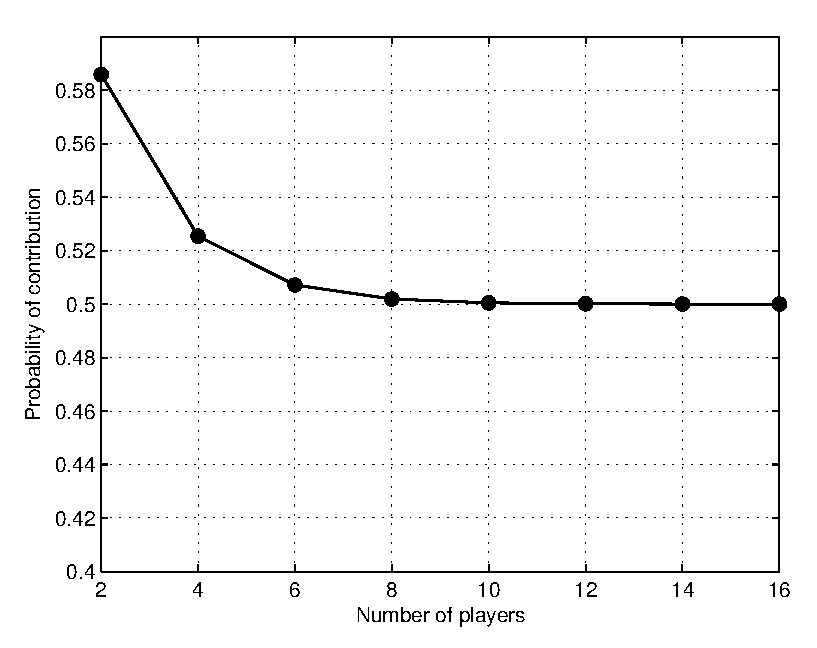
\includegraphics[scale=0.7]{../figures/bayesian_user_number_vs_contribute_probability.eps}
\caption{参与者数目与同意概率的关系}
\label{fig:bayesian_user_numb_vs_contr_prob}
\end{centering}
\end{figure}
%%%%%%%%%%%%%%%%%%%%%%%%%%%%%%%%%%%%%%%%%%%%%%%%%%%%%%%%%%%%%%%%%%%%
%%%%%%%%%%%%%%%%%%%%%%%%%%%%%%%%%%%%%%%%%%%%%%%%%%%%%%%%%%%%%%%%%%%%%
\begin{figure}[!htb]
\begin{centering}
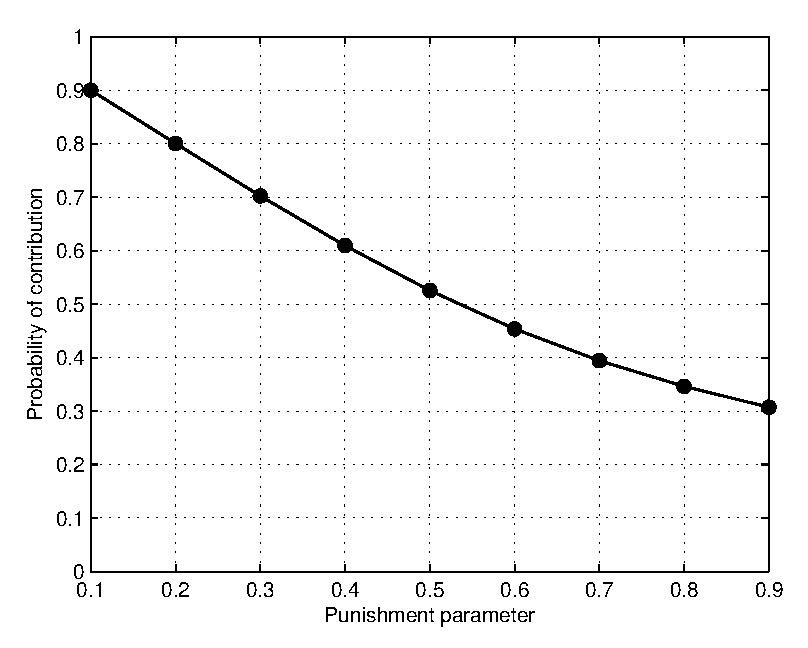
\includegraphics[scale=0.7]{../figures/bayesian_punish_parameter_vs_contribute_probability.eps}
\caption{惩罚系数与同意概率之间的关系}
\label{fig:bayesian_puni_para_vs_cont_prob}
\end{centering}
\end{figure}
%%%%%%%%%%%%%%%%%%%%%%%%%%%%%%%%%%%%%%%%%%%%%%%%%%%%%%%%%%%%%%%%%%%%
当参与者数目增多时,同意的概率会随之降低。
这意味着,当系统中参与者较少时,参与者容易做出接受资源调整的决策。
而当系统参与者较多时,即使参与者的收益比成本高,参与者也可能会做也拒绝的决定。
并且,从图中还可以看到均衡成本在参与者数目极大时,存在极限$b-\tau$。
另外,
当惩罚的系数的值增大时,并不会让参与者决定同意的机率增大。这一点与我们的直觉是不同的。
因此在系统中设置一个能够自适应网络状态的奖励参数和惩罚参数是十分必要的。
\subsection{正态分布的情况}
对于参与者的成本类型,第二种我们假设的概率分布是正态分布。
也是一个在数学、物理及工程等领域都非常重要的概率分布。
对于参与者成本随机变量$c$服从一个位置参数为$\mu$,尺度参数为$\sigma$的概率分布,
通常可以记为:
\begin{align*}
    c \sim N(\mu, \sigma^2)
    %\label{eqn:normal_distribution}
\end{align*}
服从正态分布的随机变量的概率密度函数$f(x)$由公式\ref{eqn:chap_bayesian:normoal_density}和\ref{eqn:chap_bayesian:normoal_cdf}给出,
且其概率密度函数和概率分布函数如图\ref{fig:chap_bayesian:normal_density_scheme}和\ref{fig:chap_bayesian:normal_cdf_schem}所示。
其中,与均匀分布类似的,为了将成本随机变量控制在区间$[0,1]$,我们假设成本概率分布的均值为$\mu = 0.5$,方差$\delta = 0.1$。
\begin{align}
    f(x) = \frac{1}{\sigma \sqrt{2\pi} } e^{ \frac{-(c-\mu)^2}{2\sigma^2}}
    \label{eqn:chap_bayesian:normoal_density}
\end{align}
\begin{align}
    F(x) = \frac{1}{\sigma \sqrt{2\pi} } \int^x_{-\infty}e^{ \frac{-(c-\mu)^2}{2\sigma^2}}
    \label{eqn:chap_bayesian:normoal_cdf}
\end{align}
%%%%%%%%%%%%%%%%%%%%%%%%%%%%%%%%%%%%%%%%%%%%%%%%%%%%%%%%%%%%%%%%%%%%%
\begin{figure}[tb] 
  \begin{minipage}[t]{0.5\linewidth} 
    \centering 
    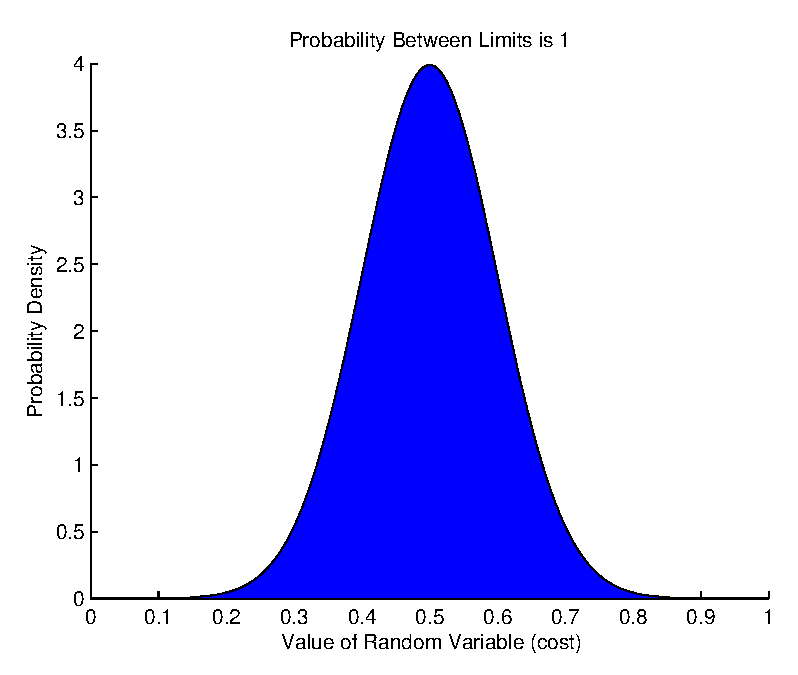
\includegraphics[width = \textwidth]{bayesian_normal_density_scheme.eps} 
    \caption{正态分布的概率密度函数} 
    \label{fig:chap_bayesian:normal_density_scheme} 
  \end{minipage}% 
  \begin{minipage}[t]{0.5\linewidth} 
    \centering 
    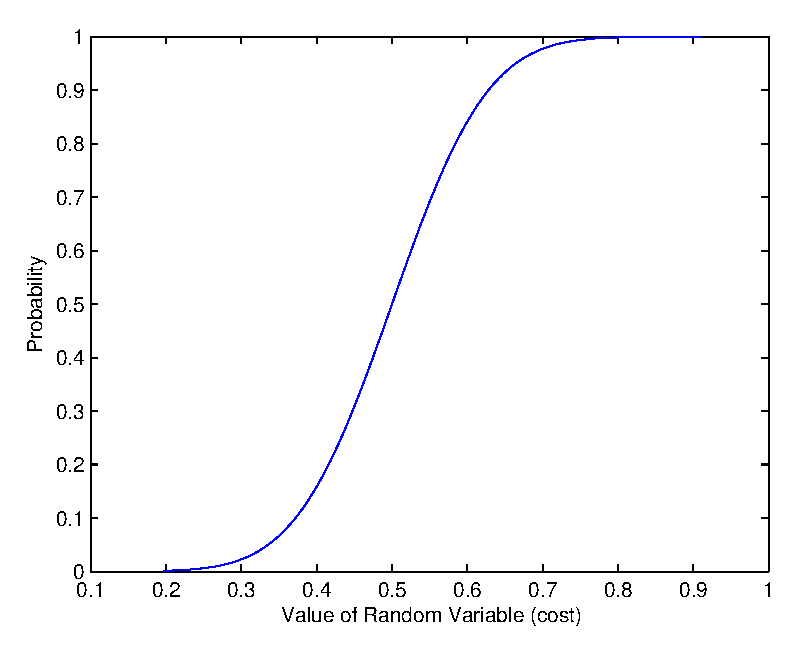
\includegraphics[width=\textwidth]{bayesian_normal_cdf_scheme.eps} 
    \caption{正态分布的累积概率函数} 
    \label{fig:chap_bayesian:normal_cdf_schem} 
  \end{minipage} 
\end{figure}
类似的,如果将公式\ref{eqn:chap_bayesian:normoal_cdf}代入公式\ref{eqn:chap_bayesian:equilibrium_cost_equation},
则有,
\begin{align} 
    c^* &= b - \tau + \left[ 1-\frac{1}{\sigma \sqrt{2\pi} } \int^x_{-\infty}e^{ \frac{-(c^*-\mu)^2}{2\sigma^2}} \right] ^{N-1}\tau
    \label{eqn:chap_bayesian:cost_normal_distribution_equation}
\end{align}
由于正态分布函数概率密度函数不能显式积分,所以我们只能通过数值求解的方式,将收益参数、惩罚参数、参与者数目与均衡概率关系画出来。
如图所示。
%%%%%%%%%%%%%%%%%%%%%%%%%%%%%%%%%%%%%%%%%%%%%%%%%%%%%%%%%%%%%%%%%%%%
\section{仿真实验与结果}

\section{小结}
